% This version is ready to be included in a group project using \include{} or \input{}
% It assumes that documentclass, packages, and global settings are handled in the main file

\begin{figure}[H]
\large
\centering
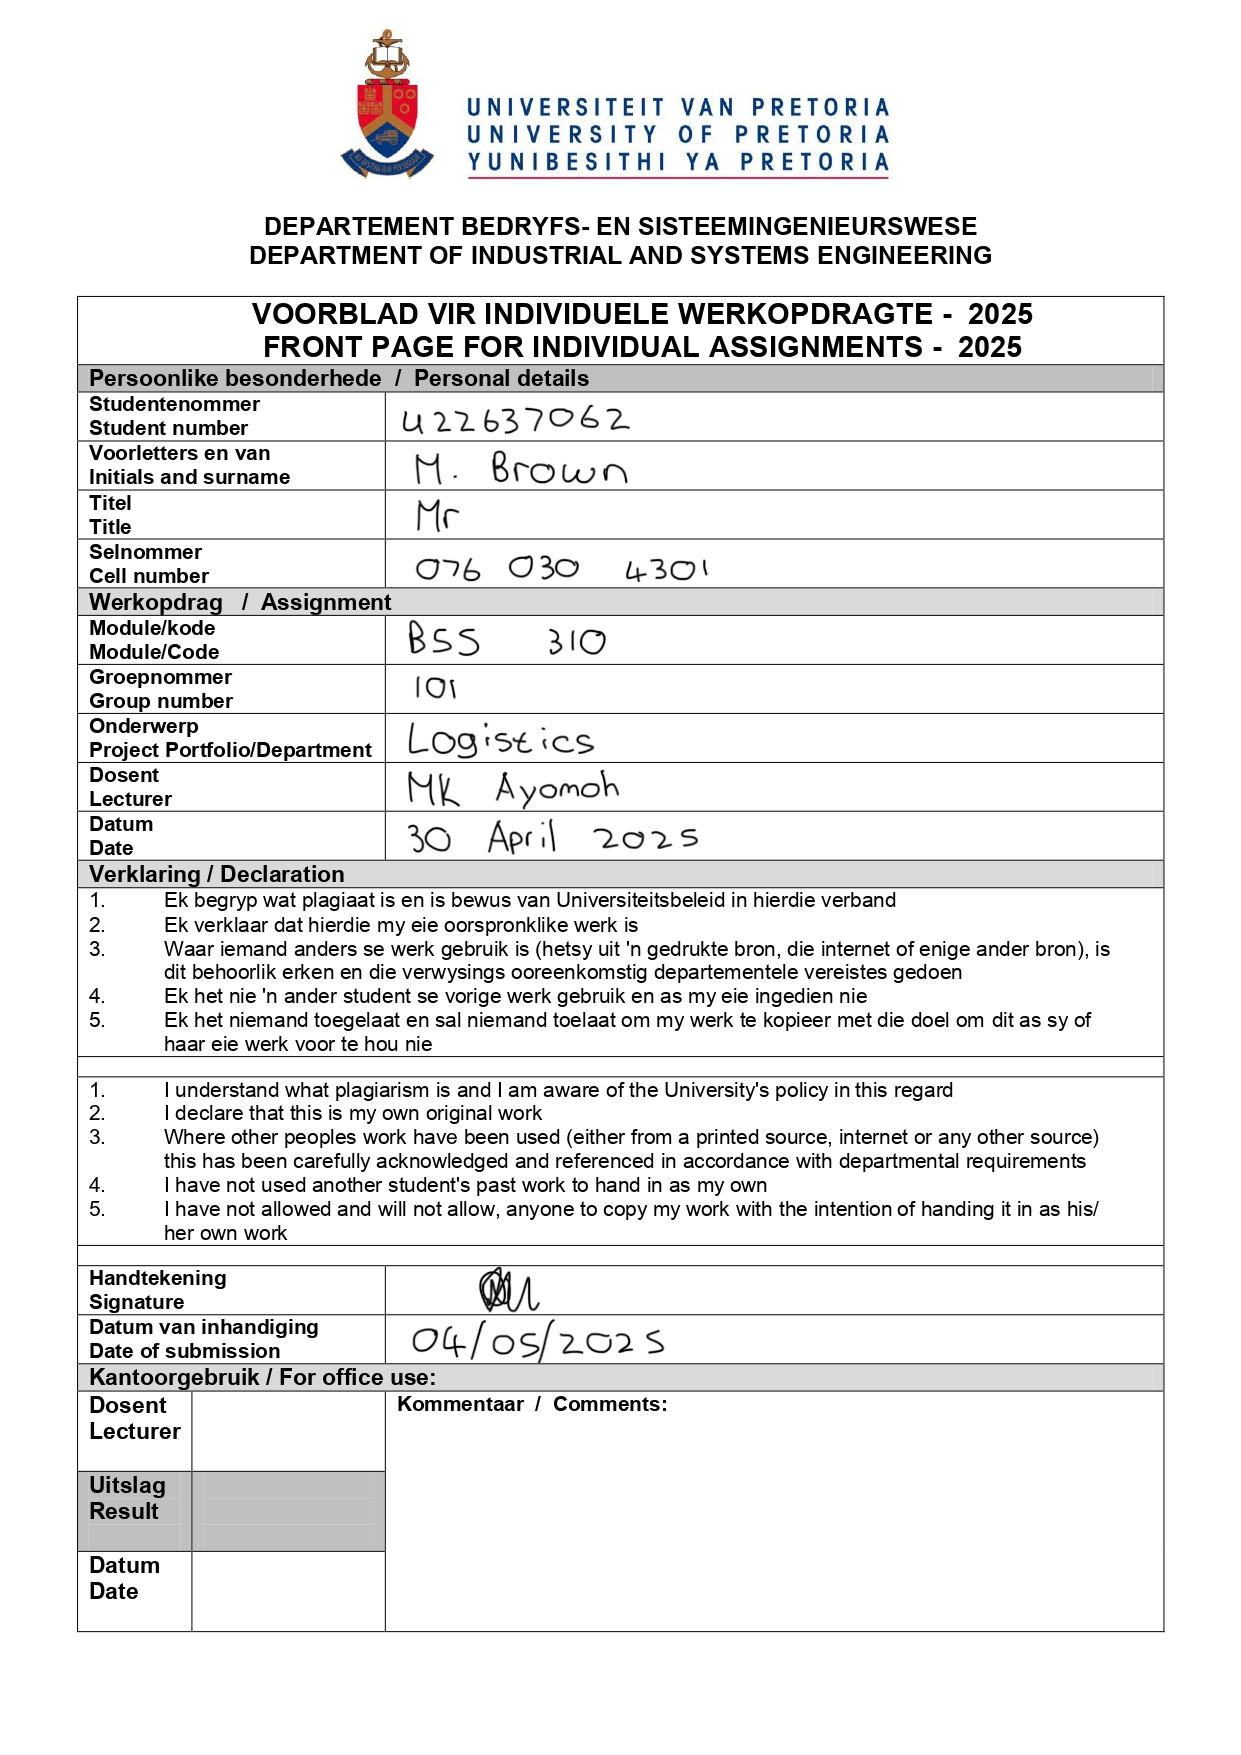
\includegraphics[width=\textwidth]{figures/Cover_Page_Part_B_Nollie.jpg}
\end{figure}

\clearpage
\large
\section{Description of System Characteristics}

The logistics system provides a quick, cost-effective and efficient flow of materials and products from suppliers to the buyers (end users), with as little as possible waste. The main functions are listed below:

\begin{itemize}[noitemsep]
  \item \textbf{Receiving and Inspection:} This characteristic includes receiving aluminium and nylon with necessary quality checks.
  \item \textbf{Inventory Control (JIT):} Only orders inventory as retail orders come in, this minimizes holding costs but a strategic safety stock is used to handle unexpected demand.
  \item \textbf{Warehousing:} A small storage room next to the manufacturing facility for raw materials and finished goods.
  \item \textbf{Distribution:} Delivery to retail and online channels (e.g., Clicks, Takealot, Dischem) is handled by 3rd party transport companies.
  \item \textbf{Forecasting:} Demand is predicted with exponential smoothing as the product might get more popular as ADHD people find out about it, thus ensuring availability without overstocking.
  \item \textbf{Labelling and Tracking:} QR codes with a video set-up guide and an inventory tracking function are used.
\end{itemize}

Together, these functions create a lean, responsive and most importantly agile supply chain aligned with the system’s objectives of affordability, portability, and professional design.

\section{Project Scope and Stakeholders}

\subsection{Project Scope}

The logistics of the project shows the strategic activities necessary to support the manufacturing and distribution of the ADHD relief seat product. This scope consists of planning, coordinating, and managing the movement and storage of raw materials and finished goods within a lean operational framework. Meaning that waste is reduced where possible and "KAIZEN" (Continuous small improvement) is applied throughout.

The primary responsibility of logistics is to ensure quick (on-time), cost-efficient, and reliable flows through all stages of the value chain — from material sourcing and initial storage set-up to final product distribution. Specific boundaries of this scope include:

\begin{itemize}[noitemsep]
  \item Overseeing contracts with aluminium and nylon suppliers
  \item Setting up a functional and minimal storage environment adjacent to the production area
  \item Implementing inventory planning strategies based on JIT principles
  \item Managing staff training and internal handling processes
  \item Coordinating with external transport providers for timely outbound deliveries
  \item Tracking logistics KPIs and improving supply responsiveness based on forecasting data
\end{itemize}

This scope supports the main objectives such as affordability, portability, and professional quality, while ensuring that all logistics activities are aligned with stakeholder expectations and delivery deadlines. The scope is fixed for the duration of the project and will be reviewed at each major phase to prevent scope creep and misalignment.

\subsection{Stakeholders}

\begin{table}[H]
\centering
\renewcommand{\arraystretch}{1.3}
\begin{tabular}{|l|l|p{6cm}|}
\hline
\textbf{Stakeholder} & \textbf{Type} & \textbf{Motivation / Role} \\
\hline
Project Group Members & Internal & Oversee design, production, logistics, and integration of subsystems. \\
\hline
Local Nylon and Aluminium Suppliers & External & Maintain steady supply at consistent quality and cost. \\
\hline
Storeroom Manager & Internal & Oversee storage, inventory replenishment, and safety stock handling. \\
\hline
Third-Party Transport Companies & External & Handle timely inbound and outbound deliveries. \\
\hline
Retail Channels (Clicks, Takealot, Dischem) & External & Distribute and promote the product to end users. \\
\hline
Retail Forecast Analysts & Internal & Predict product demand using exponential smoothing. \\
\hline
\end{tabular}
\caption{Stakeholder Roles and Responsibilities}
\end{table}

\subsection{Stakeholder Map}

\begin{figure}[H]
\centering
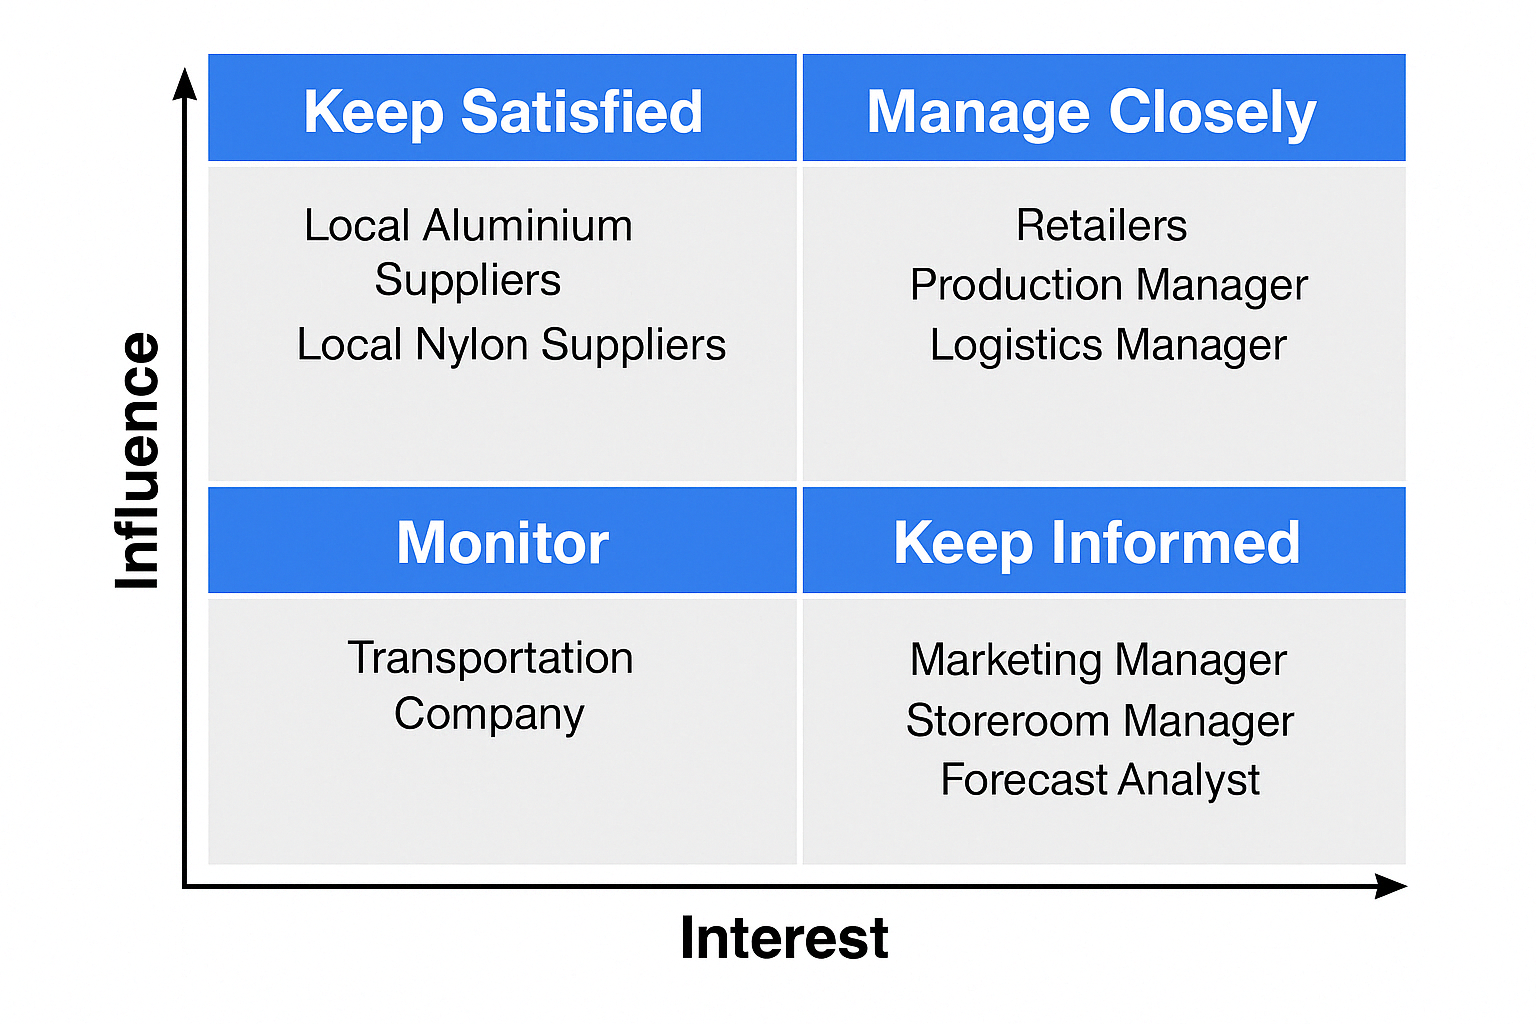
\includegraphics[width=0.6\textwidth]{figures/stakeholder_map.png}
\caption{Stakeholder Map - Interest vs Influence}
\end{figure}

\noindent High-influence stakeholders include suppliers and retailers, as they directly impact product availability and market reach.

\section{Project Plan}

\subsection{Phases and Deliverables}

\begin{table}[H]
\centering
\caption{Project Timeline and Key Deliverables}
\renewcommand{\arraystretch}{1.3}
\begin{tabular}{|p{3.5cm}|p{7.5cm}|p{3cm}|}
\hline
\textbf{Phase} & \textbf{Deliverables} & \textbf{Timeline} \\
\hline
Contracting \& Set-up &
\begin{itemize}[noitemsep, leftmargin=*]
    \item Supplier contracts finalized (aluminium and nylon)
    \item Logistics provider contracted
    \item Storage room layout completed
    \item Forecasting model and QR system installed
    \item Boot-camp training prepared
\end{itemize} &
\textbf{May 1 – May 31, 2025} \\
\hline
Execution &
\begin{itemize}[noitemsep, leftmargin=*]
    \item Raw materials delivered and then it is quality-checked
    \item Inventory system(JIT) and  processes operational
    \item Products packaged with set-up guides(QR CODES)
    \item First batch produced
\end{itemize} &
\textbf{June 1 – July 31, 2025} \\
\hline
Distribution &
\begin{itemize}[noitemsep, leftmargin=*]
    \item Stock delivered to retailers.
    \item QR-based delivery tracking implemented
    \item KPI metrics collected and evaluated
\end{itemize} &
\textbf{August 1 – August 30, 2025} \\
\hline
\end{tabular}
\end{table}

\subsection{Work Breakdown Structure (WBS)}

\begin{figure}[H]
\centering
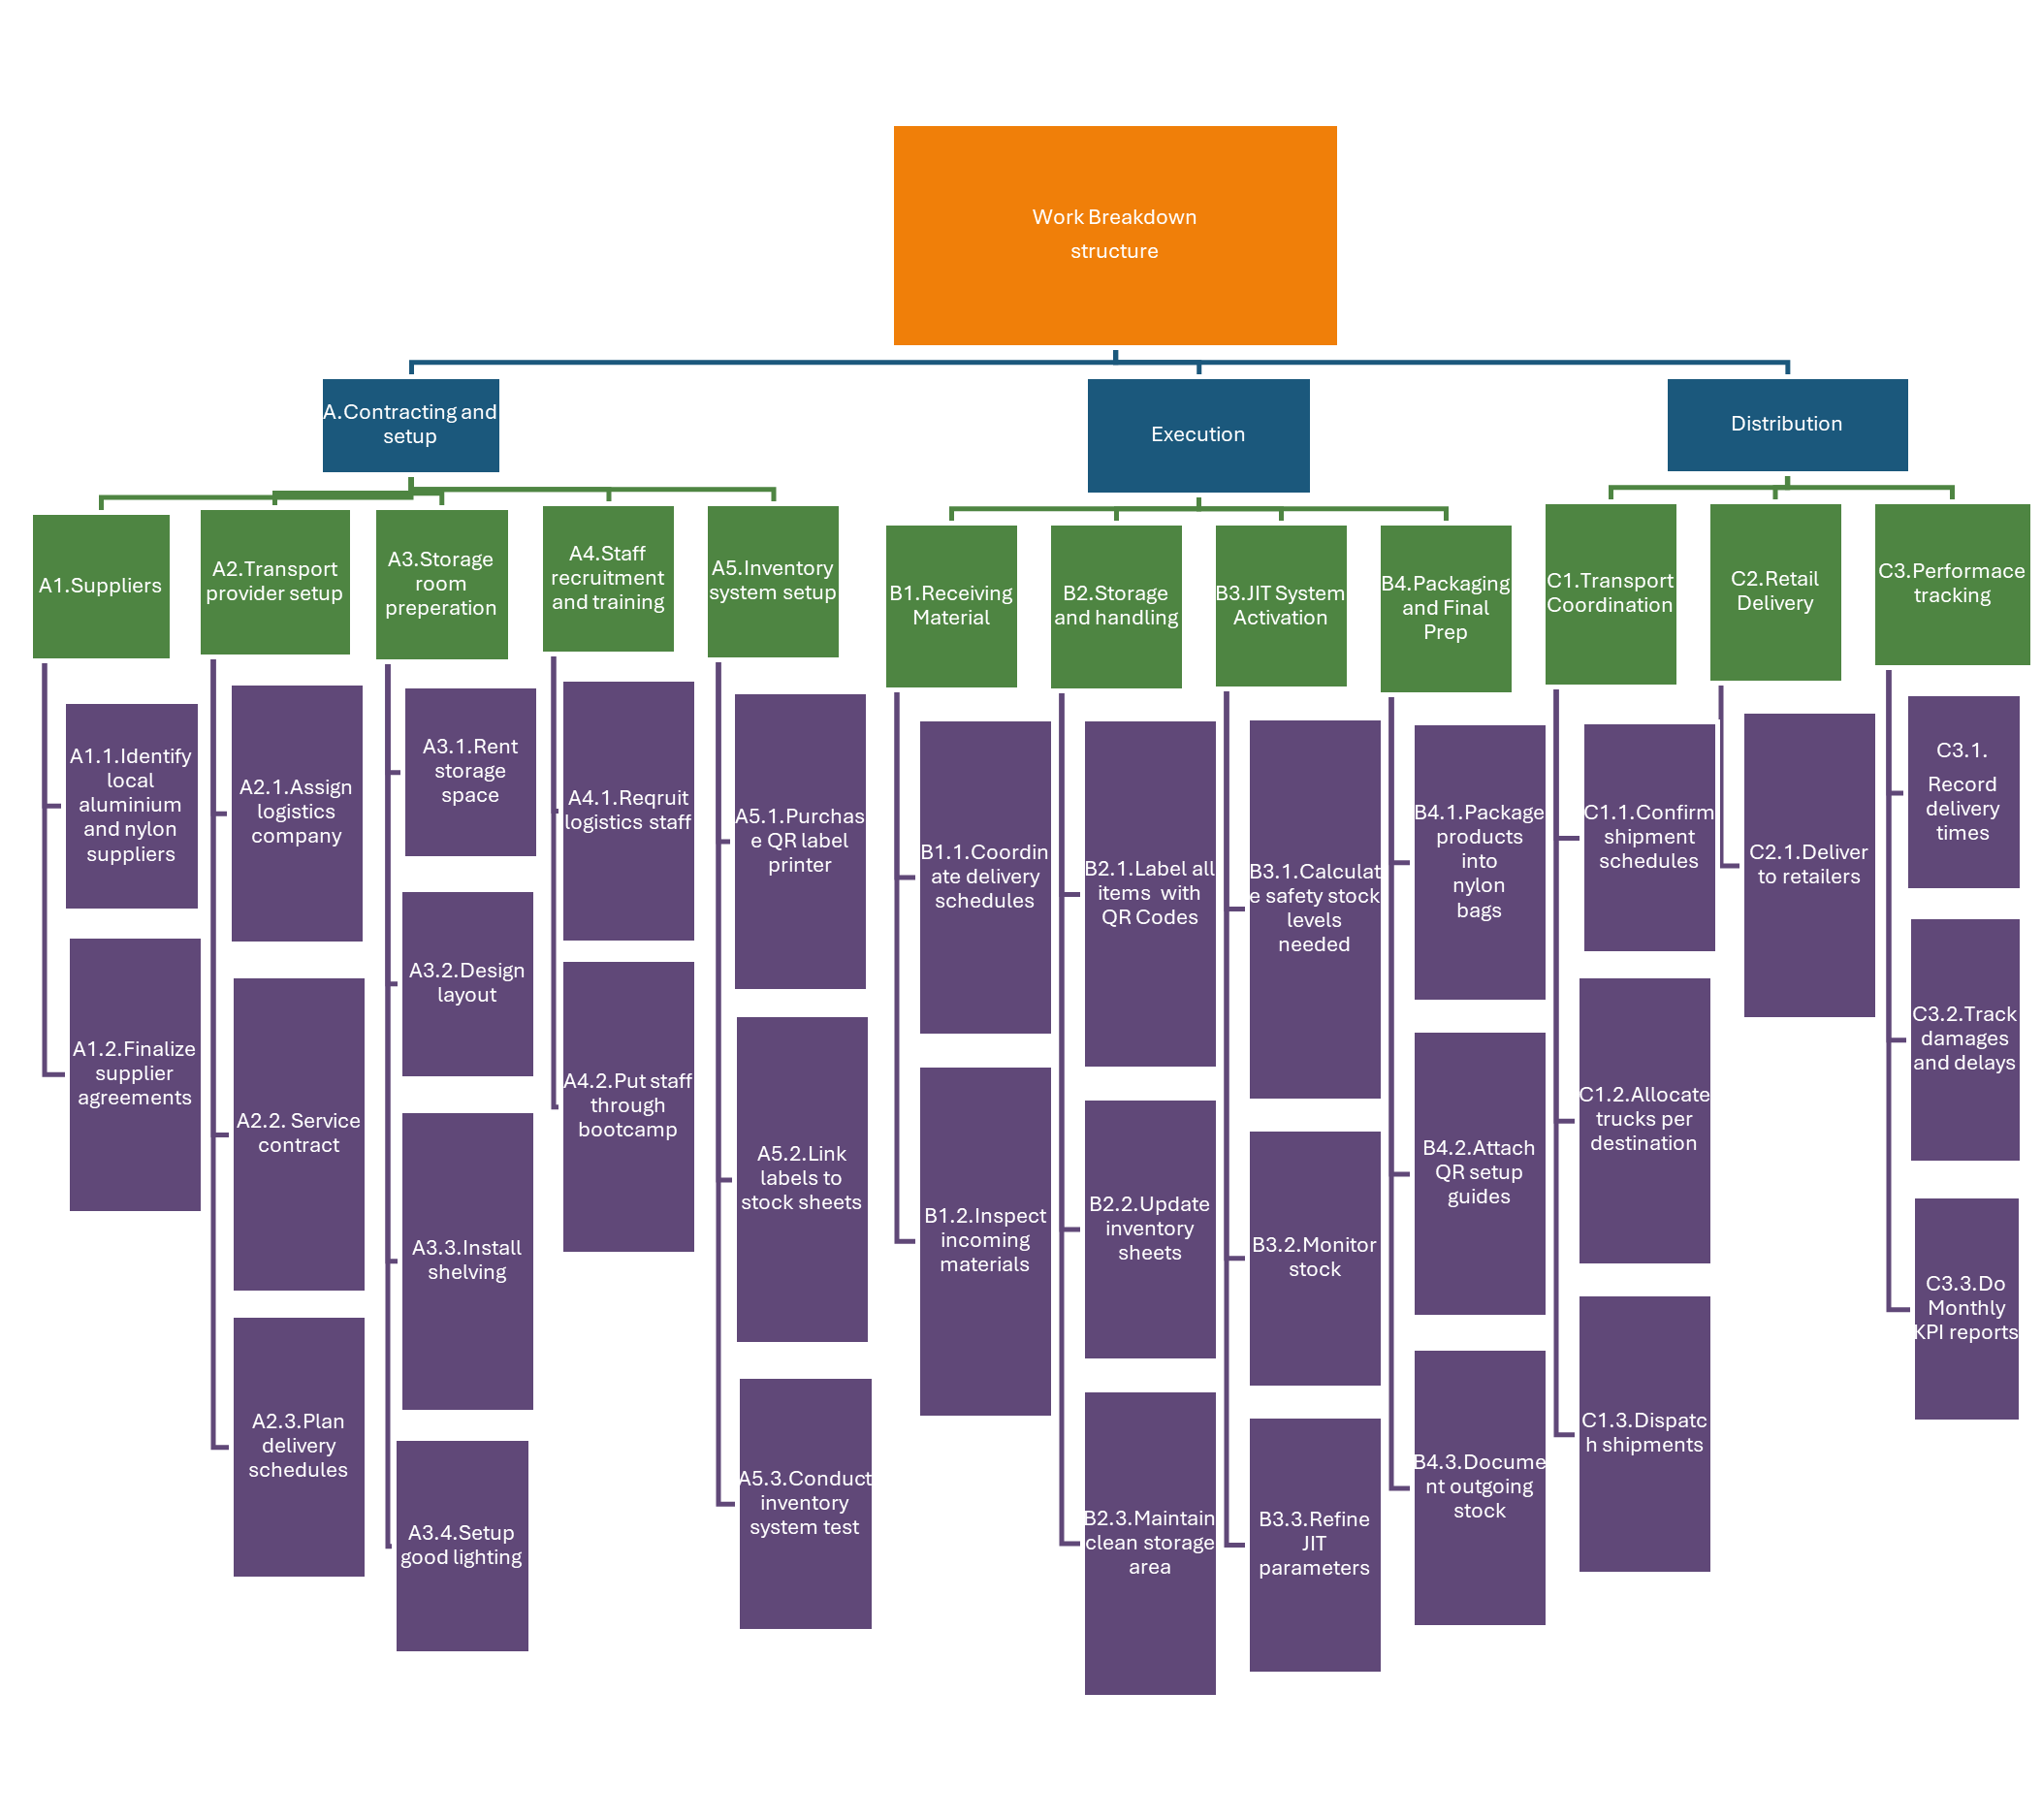
\includegraphics[width=\textwidth]{figures/Picture1.png}
\caption{Work Breakdown Structure – Logistics Subsystem}
\end{figure}

\section{Network Diagram}

\begin{figure}[H]
\centering
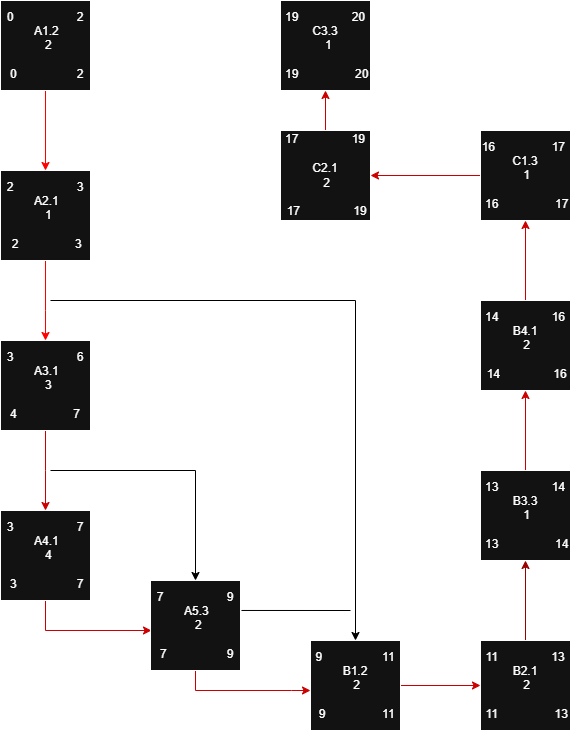
\includegraphics[width=0.85\textwidth]{figures/Network-Diagram.drawio (1).png}
\caption{Network Diagram Showing Project Activity Dependencies}
\end{figure}

\subsection{Forward and Backward Pass Summary}

\begin{table}[H]
\centering
\begin{tabular}{|l|l|}
\hline
\textbf{Forward Pass} & Start: May 1, 2025 \quad Finish: August 30, 2025 \\
\hline
\textbf{Backward Pass} & Start: May 1, 2025 \quad Finish: August 30, 2025 \\
\hline
\textbf{Project Duration} & Total Duration: 20 days (Working days) \\
\hline
\end{tabular}
\caption{Forward and Backward Pass Table}
\end{table}

\subsection{Float and Slack Table}

\begin{table}[H]
\centering
\begin{tabular}{|c|c|c|}
\hline
\textbf{Activity} & \textbf{Float (days)} & \textbf{Slack (days)} \\
\hline
A1.2 – Finalize supplier agreements & 0 & 0 \\
A2.1 – Assign logistics company & 0 & 0 \\
A3.1 – Rent storage space & 1 & 1 \\
A4.1 – Recruit/train logistics staff & 0 & 0 \\
A5.3 – Inventory system test & 0 & 0 \\
B1.2 – Inspect incoming materials & 0 & 0 \\
B2.1 – Label with QR codes & 0 & 0 \\
B3.3 – Refine JIT parameters & 0 & 0 \\
B4.1 – Package into nylon bags & 0 & 0 \\
C1.3 – Dispatch shipments & 0 & 0 \\
C2.1 – Deliver to retailers & 0 & 0 \\
C3.3 – Monthly KPI reports & 0 & 0 \\
\hline
\end{tabular}
\caption{Float and Slack for Logistics Activities}
\end{table}

\subsection{KPIs}

\begin{itemize}[noitemsep]
  \item On-time Delivery Rate $\geq$ 95\% (Ensures reliability)
  \item Inventory Turnover Rate $\geq$ 10 per annum ( Validates JIT performance)
  \item Order Accuracy $\geq$ 98\% (Tracks packing and delivery correctness)
  \item Forecast Accuracy within 10\% ( Monitors demand prediction reliability)
  \item Lead Time from supplier to factory $\leq$ 3 days ( Measures inbound efficiency)
\end{itemize}

\section{Set-Up Budget}

\begin{table}[H]
\centering
\caption{Initial Set-Up Budget for Launch Phase}
\renewcommand{\arraystretch}{1.4}
\begin{tabular}{|p{5cm}|p{7cm}|r|}
\hline
\textbf{Item} & \textbf{Description} & \textbf{Cost (R)} \\
\hline
Storage Room Setup & Shelving, layout design, lighting, and safety equipment & 50000 \\
Initial Rent & Two months' rent for temporary storage area pre-launch & 60000 \\
Forklift Lease (Deposit) & Deposit for a forklift  & 10000 \\
Boot-camp Training & 5-day skills boot-camp for logistics and stock staff (R1000/day x 4) & 20000 \\
Packaging Materials & Nylon bags and QR labels& 6000 \\
QR Label Printer & QR printer for inventory and packaging traceability & 28000 \\
Office Equipment & Basic set-up: desk, chair,multi plugs, computer, and shared printer & 10000 \\
Temporary Labour & 2 workers handling material for 20 days (R250/day each) & 10000 \\
Admin Support & 1 part-time admin for 40 days (R175/day) & 7000 \\
Transport Set-up Fee &  Agreement with transport company  & 15000 \\
\hline
\textbf{Total Set-up Cost} & & \textbf{216000} \\
\hline
\end{tabular}
\end{table}

\vspace{1em}
\noindent\textbf{Note:} Transport will be handled by a reliable and trustworthy transport company using enclosed and flatbed trucks suitable for aluminium and nylon. This means less capital is used on trucks while ensuring reliable delivery performance.

\subsection{Operational Budget (3-Year Forecast)}

\begin{table}[H]
\centering
\caption{Operational Budget for the First Three Years of Operation}
\renewcommand{\arraystretch}{1.4}
\begin{tabular}{|p{4cm}|r|r|r|r|r|}
\hline
\textbf{Expense} & \textbf{Monthly Cost} & \textbf{Year 1} & \textbf{Year 2} & \textbf{Year 3} & \textbf{3-Year Total (R)} \\
\hline
Transport Provider & R8000 & 96000 & 99000 & 102000 & 297000 \\
Logistics Manager & R6000 & 72000 & 74000 & 76000 & 222000 \\
Stock Coordinator & R4000 & 48000 & 50000 & 52000 & 150000 \\
Admin Personnel & R3500 & 42000 & 44000 & 45000 & 131000 \\
Forklift Lease & R2000 & 24000 & 12000 & 0 & 36000 \\
Maintenance & R1800 & 21600 & 22000 & 23000 & 66600 \\
Stocktaking Labour & R1800 & 21600 & 21600 & 22500 & 65700 \\
\hline
\textbf{Total} &  & 324200 & 322600 & 320500 & \textbf{967300} \\
\hline
\end{tabular}
\end{table}

\vspace{1em}
\noindent\textbf{Note:} This projection includes all key logistics, labour and operational costs. The forklift lease ends after Year 2. External transport is used to maintain good performance even if the workload gets higher.
